\subsection{Map Statistics}

Figure~\ref{fig:map-time} considers only the map tasks that fetch their data partition remotely. Note that the Map runtime includes the time to fetch the input data partition. It shows how the median runtime decreases almost exponentially as the link bandwidth is increased. Clearly there is a need to avoid these remote fetches
by preventing scheduling of map tasks on remote nodes. 
%An interesting observation is that the number of Map tasks fetching remote input decreases as the bandwidth goes down. This is a result of opportunistic scheduling in Spark since a new map task is scheduled on a core only when the previous one finishes.

\begin{figure}[!ht]
\centering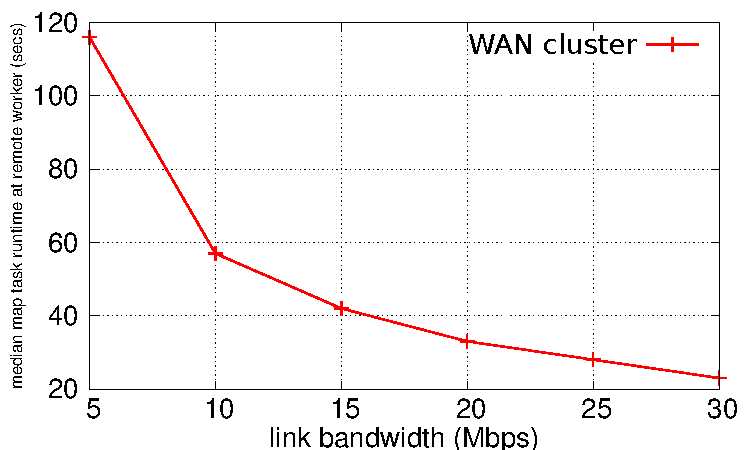
\includegraphics[width=\columnwidth]{figs/map-time.pdf}
\vspace{-1.2em}
\caption{The median execution execution time for a map task that fetches data remotely increases drastically as the wide area link bandwidth decreases.}
\label{fig:map-time}
\vspace{.7em}
\end{figure}

\subsection{Reduce Statistics}

In MapReduce and Shark, a reduce task has to fetch $M$ shuffle blocks. Some of these blocks will be local, while the rest will have to be fetched from remote nodes.  Figure~\ref{fig:reduce-blocks} shows, for each node, how the median number of remote shuffle blocks fetched by reduce tasks changes as the link bandwidth is varied. Here we see that low bandwidth causes a significant discrepancy between the number of shuffle blocks fetched remotely by the two nodes. As the bandwidth is increased, this discrepancy goes down. A higher number of remote shuffle blocks to be fetched by the reducers increases the latency, as shown in Figure~\ref{fig:reduce-time}. We see that because the reduce tasks at node 1 had to fetch a significantly higher number of shuffle blocks remotely, the median reduce runtime for node 1 is higher than node 2.   



\begin{figure}[ht]
	\centering
	\begin{minipage}[b]{0.48\linewidth}
		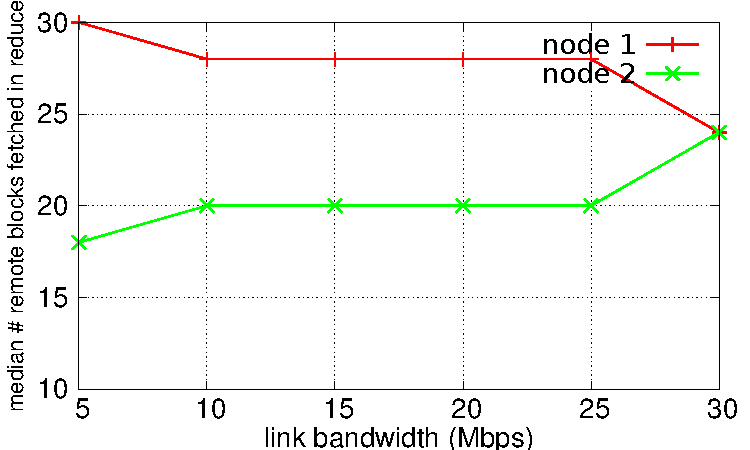
\includegraphics[width=2.5in]{figs/reduce-blocks.pdf}
		\caption{}
		\label{fig:reduce-blocks}
	\end{minipage}
	\quad
	\begin{minipage}[b]{0.48\linewidth}
		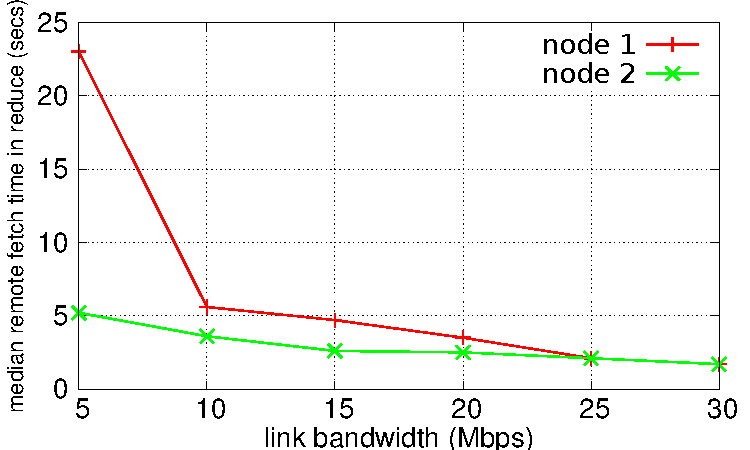
\includegraphics[width=2.5in]{figs/reduce-time.pdf}
		\caption{}
		\label{fig:reduce-time}
	\end{minipage}
\end{figure}

\subsection{Next Steps}

Our next steps are:

\begin{itemize}
\item Flesh out our designed improvements to Spark/MapReduce. As mentioned earlier, this will have two components:
\begin{itemize}
\item Run map tasks only on partitions local to a node. In other words, the Spark job is told which file resides at what node. The scheduler will then need to be modified such that each map is scheduled only for a local partition.
\item Have a sampling-based approach for fetching shuffle blocks in reduce tasks. Note that a reduce task will have to fetch a shuffle block from each map's location. Fetching all these blocks would incur a lot of overhead. Instead we plan to implement and evaluate a sampling-based approach.
\end{itemize} 
\item Evaluate our modified Spark on PageRank query
\end{itemize}

\newpage
For the PageRank query, we envision our result graphs to be like this:

\begin{figure}[ht]
	\centering
	\begin{minipage}[b]{0.48\linewidth}
		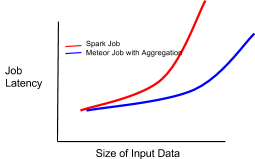
\includegraphics[width=2.5in]{figs/fig_1.png}
		\caption{Latency}
		\label{fig:minipage1}
	\end{minipage}
	\quad
	\begin{minipage}[b]{0.48\linewidth}
		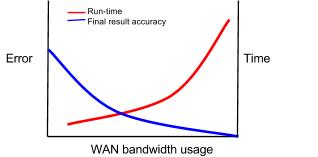
\includegraphics[width=2.5in]{figs/fig_2.png}
		\caption{Error}
		\label{fig:minipage2}
	\end{minipage}
\end{figure}

Here we increase the size of the input data on the x-axis. A Spark job with no topological awareness starts taking longer and longer since the WAN link gets saturated. On the other hand, the corresponding Meteor job takes a lot less time since it uses aggregation to reduce the data needed to be sent over the WAN link. We plan to explore how modulating the bandwidth usage over WAN affects run-time as well as final result accuracy. We expect those result to be highly dependent on the application we are targeting.

\begin{comment}
\begin{figure}[ht]
	\centering
	\begin{minipage}[b]{0.48\linewidth}
		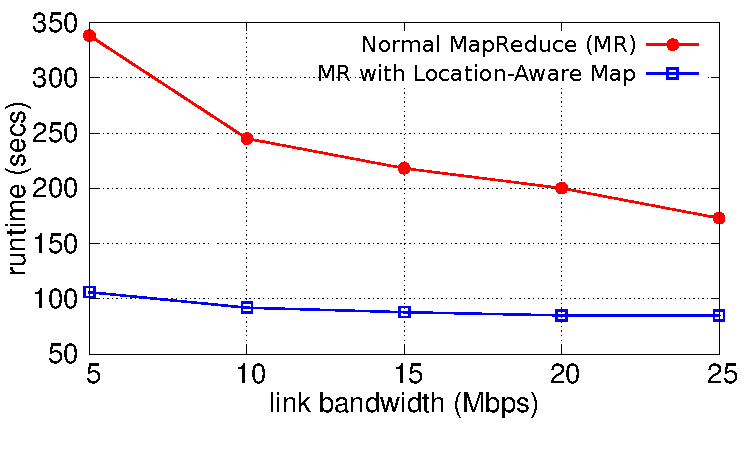
\includegraphics[width=3.5in]{figs/job-time-localMap.pdf}
		\caption{}
		\label{fig:job-time-localMap}
	\end{minipage}
	\quad
	\begin{minipage}[b]{0.48\linewidth}
		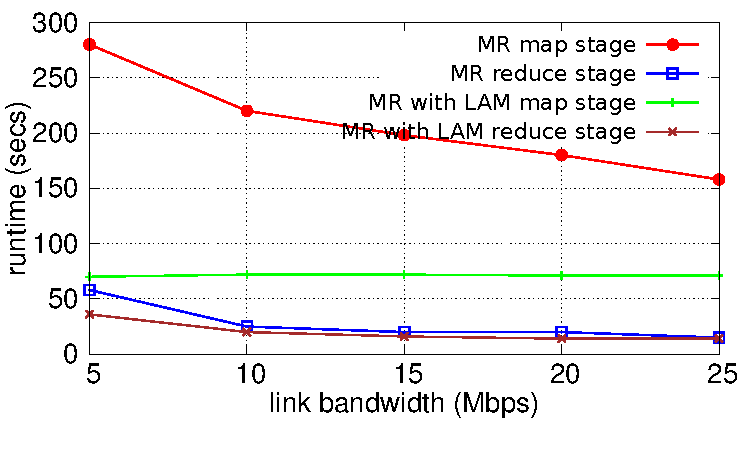
\includegraphics[width=2.5in]{figs/stage-time-localMap.pdf}
		\caption{}
		\label{fig:stage-time-localMap}
	\end{minipage}
\end{figure}
\end{comment}
